%!TeX root=../tese.tex
%("dica" para o editor de texto: este arquivo é parte de um documento maior)
% para saber mais: https://tex.stackexchange.com/q/78101

\chapter{Resultados}
\label{chap:resultados}

No capitulo \ref{chap:experimentos}, foram realizados experimentos para encontrar a combinação de 
parâmetros que proporcionava melhor desempenho para as categorias de modelos 
testadas neste estudo, regressão linear, redes \textit{feed forward}, redes
recorrentes e redes bidirecionais. Neste capítulo são apresentadas as previsões 
dos diferentes modelos.

É possível comparar o desempenho dos modelos a partir da tabela \ref{tab:compara_modelos}.

\begin{table}[H]
    \centering
    \begin{tabular}{llll}
        \toprule
        Modelo & MAE     & RMSE    & MAPE \\
        \midrule
        Regressão linear & 26435 & 38970 & 0.32  \\
        Rede \textit{feed forward} & 26880  & 50830 & 0.27 \\
        Rede recorrente & 22694 & 43918 & 0.19  \\
        \textbf{Rede bidirecional} & \textbf{19185} & \textbf{33942} & \textbf{0.17} \\
        \bottomrule
    \end{tabular}
    \caption{Comparação do desempenho dos modelos}
    \label{tab:compara_modelos}
\end{table}

Na análise da tabela acima, nota-se que o desempenho nas previsões
melhora à medida que se aumenta a robustez do modelo. A regressão linear é utilizada 
como base para avaliar o desempenho das redes neurais por ser um modelo mais 
simples. 

É possível perceber que houve uma ligeira melhora das previsões com as 
redes \textit{feed forward} em relação à regressão linear que se refletiu na 
redução do erro médio percentual
em 5\%. Essa melhora, contudo, não é perceptível nos indicadores de erro absoluto,
enquanto a MAE apresenta um valor similar que a da regressão, a RMSE teve um 
aumento significativo, isso indica a presenta de \textit{outliers}.

Observa-se uma significativa melhora de 8\% das redes \textit{feed forward} para os modelos
de redes recorrentes, reflexo da capacidade de reconhecer sequências e contexto.
A melhora também se reflete nos erros absolutos calculados pela MAE, contudo a 
RMSE apresentou piora em relação à regressão linear, provavelmente por conta 
de \textit{outliers}, uma vez que a RMSE é mais sensível a valores discrepantes.

As redes bidirecionais apresentaram melhor desempenho em comparação com os outros 
modelos, em virtude da arquitetura mais complexa com duas redes recorrentes. Há 
redução de 2\% da MAPE em relação às redes recorrentes e de 15\% em relação à 
regressão linear. Esse comportamento se reflete, também, nos indicadores de 
erro absoluto que são os menores entre as classes de algoritmos testados.

Foi adotado o estado de São Paulo para comparar as previsões  e o valor real 
do consumo, a escolha se deu por 
se tratar do maior consumidor de cimento no Brasil\footnote{Em 2019, o estado 
de São Paulo foi 
responsável por 21.3\% da demanda por cimento no Brasil, 8.6\% à frente do 
segundo maior consumidor, Minas Gerais}. A evolução do consumo 
mensal de cimento em São Paulo pode ser vista na figura \ref{consumo-sp}.

\begin{figure}[H]
    \centering
    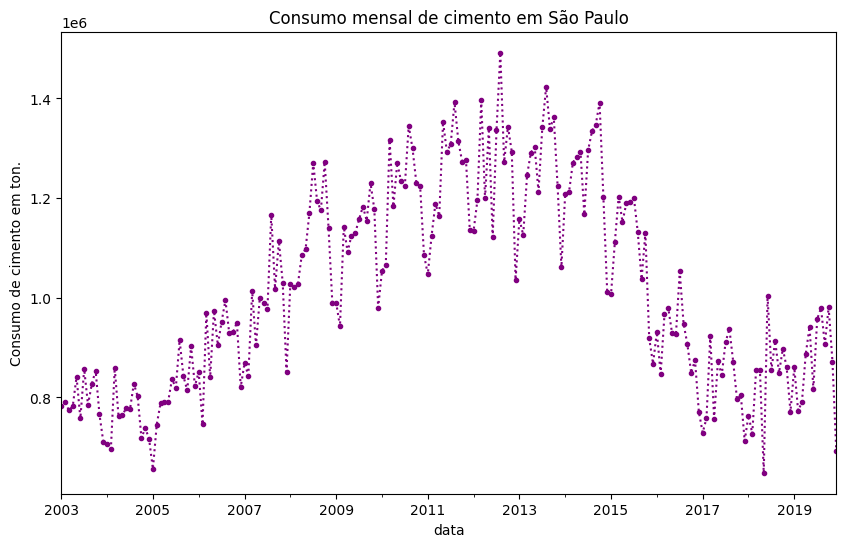
\includegraphics[width=10cm]{../figuras/graficos/evolucao-consumo-sp.png}
    \caption{Evolução do consumo mensal de cimento em São Paulo}
    \label{consumo-sp}
\end{figure}

Na imagem acima, os círculos representam as medições mensais do consumo de 
cimento em São Paulo. Observa-se que a demanda por cimento no estado vinha em tendência
de queda desde 2013 e passou a apresentar alta de 2018 em diante, além disso, há certa
sazonalidade da demanda.


\section{Regressão linear}

\begin{figure}[H]
    \centering
    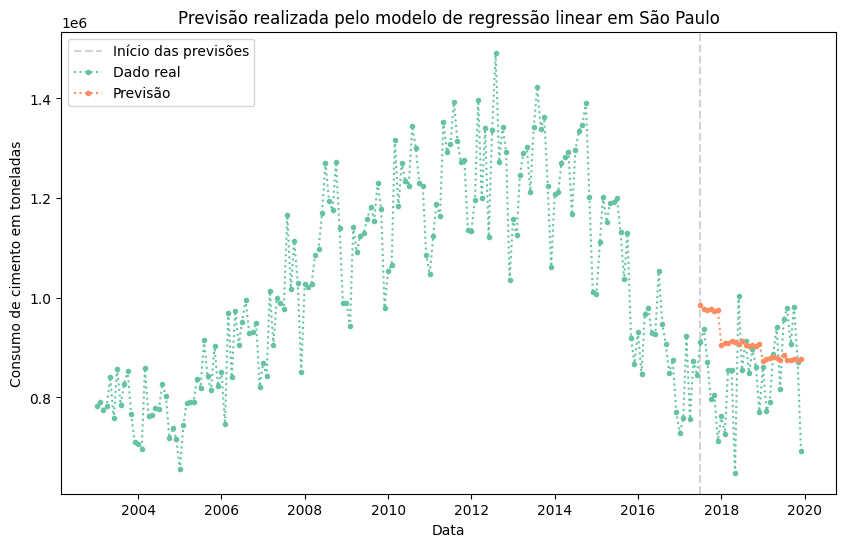
\includegraphics[width=10cm]{../figuras/graficos/reg_lin/prev_sp.png}
    \caption{Previsão realizada pela regressão linear em São Paulo}
    \label{consumo-sp}
\end{figure}

\begin{figure}[H]
    \centering
    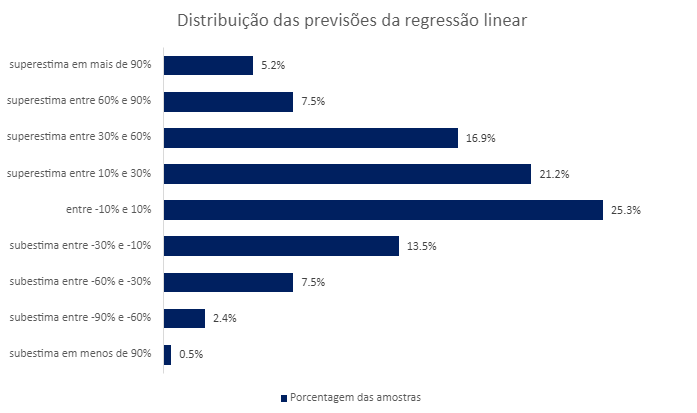
\includegraphics[width=10cm]{../figuras/graficos/reg_lin/erro-perc-rg.png}
    \caption{Previsão realizada pela regressão linear em São Paulo}
    \label{consumo-sp}
\end{figure}


\section{Redes \textit{feed forward}}

\begin{figure}[H]
    \centering
    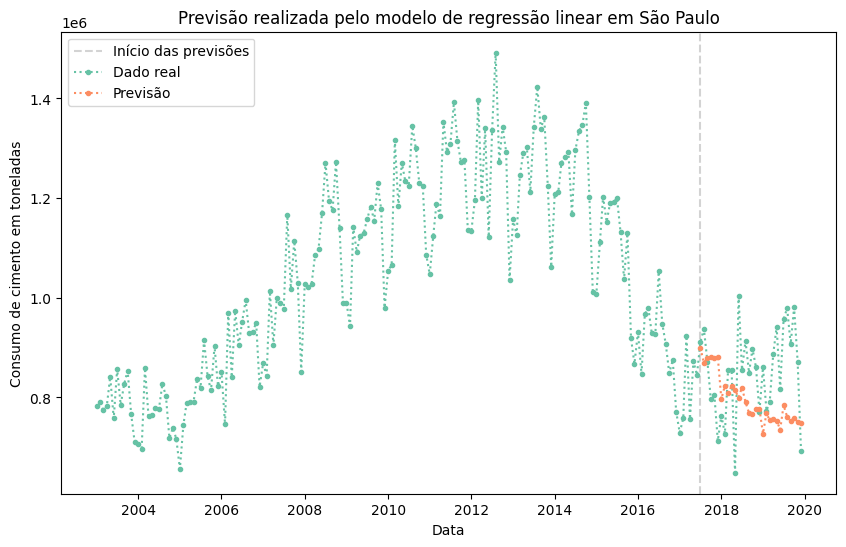
\includegraphics[width=10cm]{../figuras/graficos/mlp/prev_sp.png}
    \caption{Previsão realizada pela regressão linear em São Paulo}
    \label{consumo-sp}
\end{figure}

\begin{figure}[H]
    \centering
    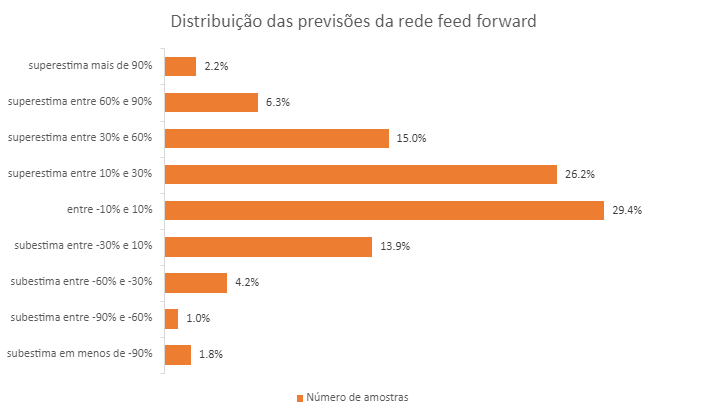
\includegraphics[width=10cm]{../figuras/graficos/mlp/erro-perc-mlp.png}
    \caption{Previsão realizada pela regressão linear em São Paulo}
    \label{consumo-sp}
\end{figure}


\section{Redes recorrentes}

\begin{figure}[H]
    \centering
    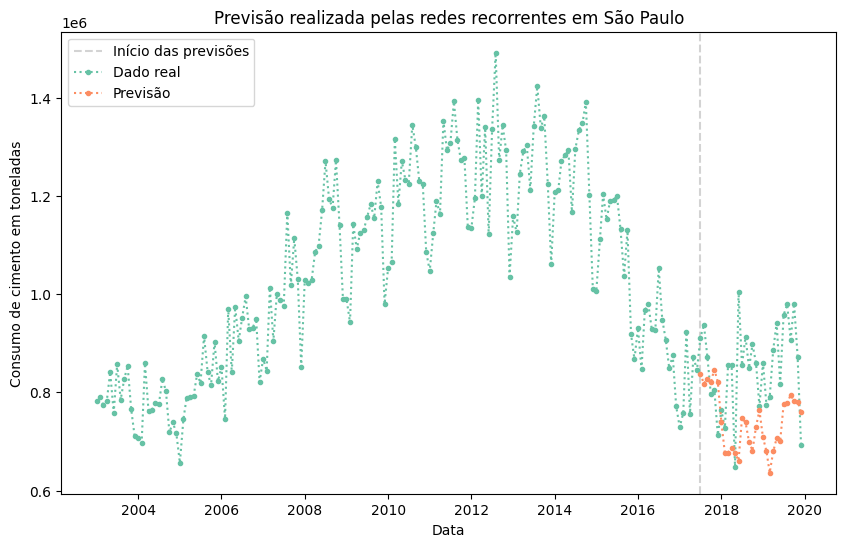
\includegraphics[width=10cm]{../figuras/graficos/rnn/prev_sp.png}
    \caption{Previsão realizada pela regressão linear em São Paulo}
    \label{consumo-sp}
\end{figure}

\begin{figure}[H]
    \centering
    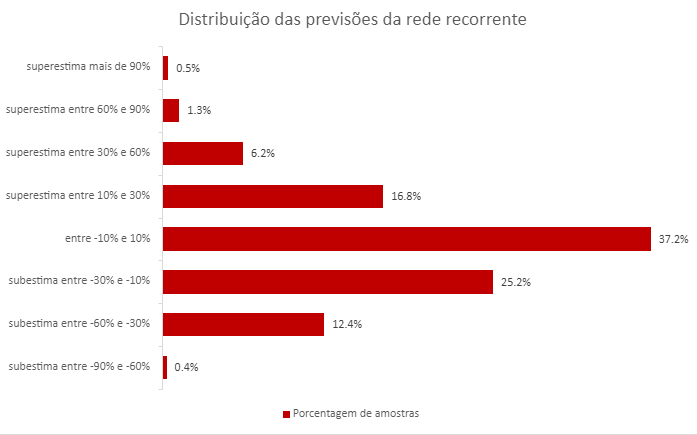
\includegraphics[width=10cm]{../figuras/graficos/rnn/erro-perc-rnn.png}
    \caption{Previsão realizada pela regressão linear em São Paulo}
    \label{consumo-sp}
\end{figure}


\section{Redes bidirecional}

\begin{figure}[H]
    \centering
    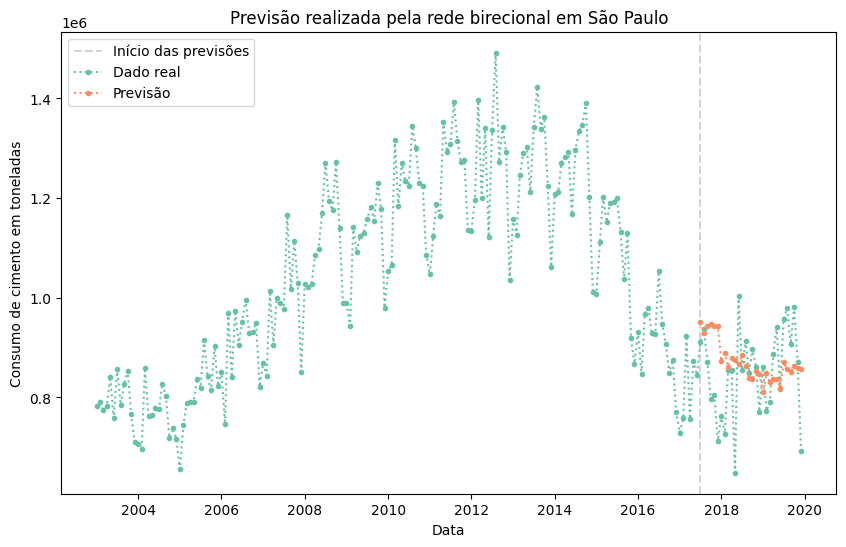
\includegraphics[width=10cm]{../figuras/graficos/bi/prev-sp-bi.png}
    \caption{Previsão realizada pela regressão linear em São Paulo}
    \label{consumo-sp}
\end{figure}

\begin{figure}[H]
    \centering
    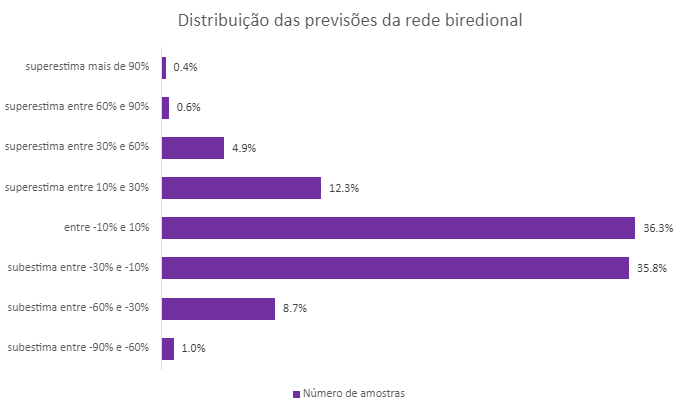
\includegraphics[width=10cm]{../figuras/graficos/bi/erro-perc-bi.png}
    \caption{Previsão realizada pela regressão linear em São Paulo}
    \label{consumo-sp}
\end{figure}